% (c) 2012 - 2014 - Dimitrios Vrettos d.vrettos@gmail.com
% (c) 2014 Daniele Zambelli - daniele.zambelli@gmail.com

\chapter{Sistemi di equazioni}

\section{Equazione lineare in due incognite}
\label{sec:sist_eqdue}

\begin{definizione}
Una equazione di primo grado in due incognite si chiama \emph{equazione 
lineare}.
\end{definizione}

\begin{problema}
Determinare due numeri naturali la cui somma sia~16.
\end{problema}

\begin{soluzione}
L'ambiente del problema è l'insieme~$\insN$ dei numeri naturali. Indicati 
con~$x$ e~$y$ i due numeri
richiesti dal quesito, il problema si formalizza con l'equazione~$x+y=16$, 
equazione in due incognite, di
primo grado.

Determiniamo l'Insieme Soluzione del problema proposto.
L'obiettivo è trovare~$x\in\insN$ e~$y\in\insN$ tali che~$x+y=16$ 
oppure~$(x;y)\in\insN\times\insN$ tali che~$x+y=16$.
Le coppie di numeri naturali che sono soluzioni
dell'equazione sono facilmente determinabili e sono
tutte quelle riportate nella tabella seguente.

\begin{tabular}{cccccccccccccccccccc}
\toprule
$x$ & 0 & 1 & 2 & 3 & 4 & 5 & 6 & 7 & 8 & 9 & 10 & 11 & 12 & 13 & 14 & 15 & 16\\
$y$ & 16 & 15 & 14 & 13 & 12 & 11 & 10 & 9 & 8 & 7 & 6 & 5 & 4 & 3 & 2 & 1 & 0\\
\bottomrule
\end{tabular}

L'Insieme Soluzione del problema posto è dunque
formato dalle~17 coppie di numeri naturali sopra elencate.
Riformuliamo il problema cercando coppie di numeri razionali la cui
somma sia~16.
In simboli scriviamo~$x\in\insQ$ e~$y\in\insQ$ tali che~$x+y=16$ 
oppure~$(x;y)\in\insQ\times\insQ$ tali che~$x+y=16$.

Possiamo subito dire che tutte le coppie precedenti sono soluzione del
problema, ma ce ne sono infinite altre, ad esempio la coppia~$(-7;+23)$ è 
soluzione del problema perché sostituendo a~$x$ il
valore~$-7$ e a~$y$ il valore~$+23$ si ha~$(-7)+(+23)=16$.
Dal procedimento si capisce che anche la coppia~$(+23;-7)$ è
soluzione del problema perché~$(+23)+(-7)=16$.

Se attribuiamo un valore arbitrario a~$x$, l'altro
elemento della coppia soluzione si può ottenere sottraendo da~16 il
valore di~$x$:~$y=16-x$.

Completa tu:

\begin{itemize}
\item se~$x=-3$ allora~$y=16-(-3)=\ldots\ldots$ e la coppia (\ldots; \ldots) è 
soluzione dell'equazione;
\item se~$x=\frac{3}{2}$ allora~$y =\dotfill$, la coppia (\ldots\ldots; 
\ldots\ldots) è soluzione dell'equazione;
\item se~$x =\dotfill$ allora~$y=$ \dotfill, la coppia (\ldots\ldots; 
\ldots\ldots) è soluzione dell'equazione;
\item se~$x=\dotfill$allora~$y =$ \dotfill, la coppia (\ldots\ldots; 
\ldots\ldots) è soluzione dell'equazione.
\end{itemize}

Quindi, se l'ambiente del problema è
l'insieme~$\insQ$, troviamo infinite coppie di
numeri razionali che soddisfano il problema.
E ancora, se formuliamo il problema nell'insieme dei
numeri reali~$\insR$, troveremo tutte le infinite coppie
soluzione del problema: basta assegnare all'incognita~$x$
valori reali arbitrari e determinare di conseguenza il corrispondente
valore di~$y=16-x$.

Se~$x=\sqrt{2}\Rightarrow y=16-\sqrt{2}$, la 
coppia~$\left(\sqrt{2};16-\sqrt{2}\right)$ è soluzione
dell'equazione. 

% \newpage %------------------------------------------------------

Completa:

\begin{itemize}
\item se~$x=-2\sqrt{3}+1$ allora~$y=\dotfill$
\item se~$x=16+\frac{3\sqrt{5}}{2}$ allora~$y=\dotfill$
\end{itemize}
\end{soluzione}

\begin{definizione}
Si chiama \emph{Insieme Soluzione} $(\IS)$ di un'equazione di primo
grado in due incognite, l'\emph{insieme delle coppie
ordinate} di \emph{numeri reali} che sostituiti rispettivamente a~$x$ e
a~$y$ rendono vera l'uguaglianza.
\end{definizione}

% \ovalbox{\risolvii \ref{ese:22.1}, \ref{ese:22.2}, \ref{ese:22.3}}

\subsection{Rappresentazione di un'equazione lineare sul piano cartesiano}

% \begin{exrig}\vspace{1.10ex}
 \begin{esempio}
Determinare l'insieme soluzione dell'equazione~$3y-x+1=0$ con~$x\in\insR$ 
e~$y\in\insR$.
 \end{esempio}
Osserviamo che l'equazione assegnata ha due incognite ed
è di primo grado; l'insieme soluzione sarà formato
dalle infinite coppie ordinate~$(x;y)$ di numeri tali che~$3y-x+1=0$.

Possiamo verificare che la coppia~$(1;0)$ è soluzione
dell'equazione, ma come facciamo a determinare tutte le
coppie che soddisfano quella equazione?

Fissiamo l'attenzione sull'incognita~$y$,
pensiamo l'equazione come un'equazione
nella sola~$y$, ricaviamo~$y$ come abbiamo fatto nelle equazioni di primo
grado ad una sola incognita, applicando i principi di equivalenza delle
equazioni:

\begin{equation*}
3y-x+1=0\Rightarrow~3y=x-1\Rightarrow\frac{3y}{3}=\frac{x-1}{3}\Rightarrow 
y=\frac{1}{3}x-\frac{1}{3}.
\end{equation*}
Al variare di~$x$ in~$\insR$, si ottengono tutte le infinite
soluzioni dell'equazione assegnata.
Prova a determinarne alcune:
\begin{center}
 \begin{tabular}{ccc}
\toprule
x & y & coppia\\
\midrule
$0$ &\ldots\ldots & ($0$\ldots\ldots)\\
1& \ldots\ldots &($1$\ldots\ldots)\\
$-1$ & \ldots\ldots & ($-1$\ldots\ldots)\\
\bottomrule
\end{tabular}
\end{center}

In verità non possiamo trovare tutte le infinite coppie che risolvono
quella equazione, ma possiamo darne una rappresentazione grafica.

\begin{wrapfigure}{o}{0pt}
 % (c) 2012 Dimitrios Vrettos - d.vrettos@gmail.com
\begin{tikzpicture}[font=\small,x=5mm, y=5mm]

\draw[help lines,orange, dotted] (-3,-3) grid [step=1](5,5);

\begin{scope}[thick,->]
\draw (0,-3) -- (0,5);
\draw (-3,0) -- (5,0);
\end{scope}

\end{tikzpicture}
\end{wrapfigure}

La formula \[y=\frac{1}{3}x-\frac{1}{3}\] rappresenta una funzione
lineare; riportiamo le coppie trovate in un riferimento cartesiano
ortogonale e tracciamo la retta che rappresenta la funzione.

Una qualunque equazione lineare~$ax+by+c=0$ ammette infinite
soluzioni, costituite da coppie ordinate di numeri reali; esse sono le
coordinate cartesiane dei punti della retta grafico della 
funzione~$y=-{\frac{a}{b}}x-\frac{c}{b}$.
La formula~$y=-{\frac{a}{b}}x-\frac{c}{b}$ si chiama \emph{equazione esplicita 
della retta}.

\begin{esempio}
 Risolvi graficamente l'equazione~$y+\frac{2}{3}x-2=0\text{, con 
}x\in\insR\text{ e }y\in\insR$.
\end{esempio}

\begin{wrapfloat}{figure}{r}{0pt}
% (c) 2012 Dimitrios Vrettos - d.vrettos@gmail.com
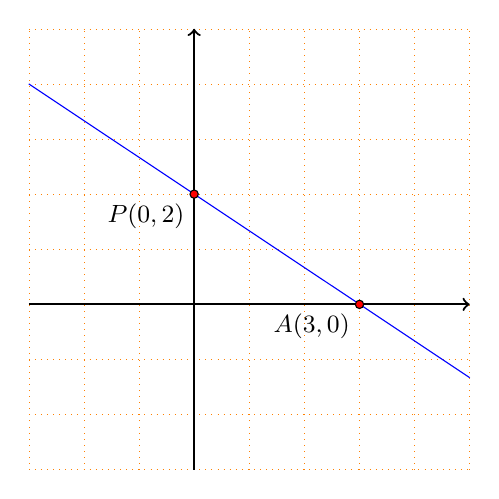
\begin{tikzpicture}[font=\small,x=7mm, y=7mm]

\draw[help lines,orange, dotted] (-3,-3) grid [step=1](5,5);

\begin{scope}[thick,->]
\draw (0,-3) -- (0,5);
\draw (-3,0) -- (5,0);
\end{scope}

\draw[blue] (-3,4) -- (5,-1.33);

\draw[fill=red] (0,2) circle (1.5pt) node[below left] {$P(0,2)$};
\draw[fill=red] (3,0) circle (1.5pt) node[below left] {$A(3,0)$};
\end{tikzpicture}
\end{wrapfloat}

L'equazione assegnata è in due incognite, di primo
grado, è cioè una equazione lineare. Nel riferimento cartesiano
ortogonale essa rappresenta una retta.

Troviamo l'equazione esplicita della retta:
\[y+\frac{2}{3}x-2=0\Rightarrow y=-{\frac{2}{3}}x+2.\]

Individuiamo l'ordinata del punto di intersezione della
retta con l'asse~$y$:~$q=2$, quindi~$P(0;2)$ è un
punto della retta.

Troviamo un altro punto appartenente alla retta: se~$x=3$ allora~$y=0$,
quindi~$A(3;0)$ è un punto della retta.

Disegniamo la retta nel piano cartesiano: le coppie~$(x;y)$, coordinate
dei punti della retta tracciata, sono le infinite soluzioni
dell'equazione assegnata.\vspace{1.10ex}
% \end{exrig}

% \ovalbox{\risolvii \ref{ese:22.4}, \ref{ese:22.5}, \ref{ese:22.6}}

\section{Definizione di sistema di equazioni}
\label{sec:sist_definizione}

\begin{problema}
\label{pr:22.1}
Nel rettangolo~$ABCD$, la somma del doppio dell'altezza con la metà della base
è di~$98\unit{m}$ aumentando l'altezza di~$3\unit{m}$ e la base di~$2\unit{m}$ 
il perimetro del rettangolo diventa di~$180\unit{m}$. 
Determinare l'area in~$\unit{m}^{2}$ del rettangolo.
\end{problema}
\begin{multicols}{2}
\emph{Dati}:
\begin{align*}
&2\overline{AD}+\frac{1}{2}\overline{AB}=98\unit{m},\\
&2(\overline{AD}+3m+\overline{AB}+2m)=180\unit{m}.
\end{align*}

\emph{Obiettivo}: Area

\begin{center}
\begin{inaccessibleblock}[Rettangolo ABCD]
 % (c) 2012 Dimitrios Vrettos - d.vrettos@gmail.com
\begin{tikzpicture}[font=\small,x=2mm, y=2mm]
	\draw (0,0) rectangle  (9.6,7.4);

\node [below left] at (0,0) {$A$};
\node[below right]  at (9.6,0) {$B$};
\node[above right]  at (9.6,7.4) {$C$};
\node[above left]  at (0,7.4) {$D$};
\end{tikzpicture}
 \end{inaccessibleblock}
\end{center}
\end{multicols}

Per determinare l'area del rettangolo dobbiamo moltiplicare le misure 
delle sue dimensioni~$\Area=\overline{AB}\cdot\overline{BC}$
che però non conosciamo; il problema ha quindi due incognite.

Analizzando i dati possiamo osservare che ci sono fornite due
informazioni che legano le grandezze incognite. 
Se poniamo~$\overline{AD}=x$ e~$\overline{AB}=y$
otteniamo le due equazioni:
\[2x+\frac{1}{2}y=98;\quad~2(x+3+y+2)=180\]
che dovranno risultare soddisfatte per una stessa coppia di numeri
reali.

\begin{osservazione}
 Dobbiamo tenere presente che questa sostituzione produce delle equazioni 
 che potrebbero avere come soluzione dei numeri negativi, mentre nel problema 
 di partenza non ha senso un rettangolo con lati di lunghezza negativa.
 Quindi:~$x \geqslant 0 \text{ e } y \geqslant 0$
\end{osservazione}

\begin{definizione}
Si definisce \emph{sistema di equazioni} l'insieme di più equazioni, 
in due o più incognite,
che devono essere verificate contemporaneamente. La scrittura formale
si ottiene raggruppando le equazioni mediante una parentesi graffa.
\end{definizione}

Il problema \ref{pr:22.1} si formalizza dunque con il sistema:
\[\longarray\left\{\begin{array}{l}
 2x+\dfrac{1}{2}y=98 \\
 2(x+3+y+2)=180
\end{array}\right.\]

\begin{definizione}
L'Insieme Soluzione ($\IS$) di un sistema di equazioni in
due incognite è formato da tutte le coppie di numeri reali
che rendono vere tutte le equazioni
contemporaneamente.
\end{definizione}

\begin{definizione}
Si chiama \emph{grado di un sistema} il prodotto dei gradi delle
equazioni che lo compongono. In particolare, se le equazioni che lo
compongono sono di primo grado, il sistema si chiama \emph{sistema lineare}.
\end{definizione}

\begin{definizione}
Un sistema si dice scritto in \emph{forma normale} o \emph{canonica} 
quando in ogni equazione tutti i monomi che contengono le incognite sono 
scritti nel primo membro e in ordine:
\[\left\{\begin{array}{l}
 a_{0}x+b_{0}y=c_{0} \\
 a_{1}x+b_{1}y=c_{1} 
\end{array}\right.
\text{ con }a_{0}, b_{0}, c_{0}, a_{1}, b_{1}, c_{1}\text{ numeri reali.}\]
\end{definizione}

Il sistema a cui si giunge risolvendo il problema posto all'inizio è
composto da due equazioni in due incognite, è di primo grado 
e quindi è un sistema lineare. 
La sua forma canonica si ottiene sviluppando i calcoli:

\[\left\{\begin{array}{l}
4x+y=196\\
x+y=85
\end{array}\right.\]

Nel seguito vedremo in particolare come risolvere sistemi lineari 
di due equazioni in due incognite.

\section{Metodi di soluzione di sistemi di equazioni}
\label{sec:sist_soluzione}

Per risolvere un sistema conviene sempre, come primo passo scriverlo in forma 
normale.

\subsection{Procedimento per ottenere la forma canonica di un sistema}
Per ottenere la \emph{forma canonica} di un sistema lineare dobbiamo:
\begin{enumerate*}
 \item spostare tutti i termini che contengono incognite a primo membro;
 \item spostare i termini senza incognite a secondo membro;
 \item ordinare i monomi con le incognite.
\end{enumerate*}

% \begin{exrig}
 \begin{esempio}
 Scrivere in forma canonica il sistema:
\[\longarray\left\{\begin{array}{l}4x^{2}-(y+2x)^{2}=x+1-y(4x+y-1)\\
\dfrac{x-2}{2}+\dfrac{y+3}{3}=0
\end{array}\right.\]

Eseguiamo i calcoli nella prima equazione e riduciamo allo stesso
denominatore la seconda equazione:

\[\left\{\begin{array}{l}
 4x^{2}-y^{2}-4x^{2}-4xy=x+1-4xy-y^{2}+y\\
 3x-6+2y+6=0
 \end{array}\right.\]

Per mezzo del primo principio di equivalenza delle equazioni portiamo le
incognite al primo membro e sommiamo i termini simili:
 \[\left\{\begin{array}{l}
   x+y=-1\\
   3x+2y=0
\end{array}\right.\]
che è la forma canonica cercata.
 \end{esempio}
% \end{exrig}


\subsection{Sistemi indeterminati o impossibili}

Prima di utilizzare uno dei metodi di soluzione che saranno descritti più 
avanti, conviene riflettere su alcuni casi particolari. Consideriamo il 
seguente sistema:

\[\sistema{3x +7y = 9 \\ 3x +7y = 10}\]

È abbastanza ovvio che la stessa espressione non possa valere 
contemporaneamente sia~9 sia~10. Questo sistema è \emph{impossibile}.

Osserviamo anche quest'altro caso:

\[\sistema{5x +8y = 17 \\ 5x +8y = 17}\]

Questa volta possiamo osservare che non abbiamo una sistema di \emph{due} 
equazioni, ma un sistema con una sola equazione ripetuta due volte. In questo 
caso, come già visto, l'equazione ha infinite soluzioni e si dirà 
\emph{indeterminato}.

Ora, se non ci troviamo in una di queste due situazioni, possiamo cercare dei 
modi per trovare l'unica soluzione del sistema.

\subsection{Metodo di sostituzione}
\emph{Risolvere il sistema} significa determinare tutte le coppie di
numeri reali che soddisfano contemporaneamente le due equazioni.

Analizziamo i diversi metodi che permettono di ottenere
l'Insieme Soluzione, cominciamo dal \emph{metodo di sostituzione}.

% \begin{exrig}
\begin{esempio}
$\left\{\begin{array}{l}-3x+y=2\\5x-2y=7\end{array}\right.$.
\end{esempio}

Il sistema si presenta già in forma canonica. Il metodo di
sostituzione si svolge nei seguenti passi:

\begin{enumerate}
 \item Scegliamo con intelligenza una delle due equazioni e una
delle due incognite da cui partire. 
La furbizia consiste nello scegliere una incognita con il coefficiente uguale 
a~$1$ o~$-1$.
Applicando i principi d'equivalenza delle equazioni, ricaviamo questa
incognita.
Nel nostro esempio, partiamo dalla prima equazione e ricaviamo
l'incognita~$y$:
\[\left\{\begin{array}{l}
     -3x+y=2\\
     5x-2y=7
    \end{array}
\right.
\Rightarrow
\left\{\begin{array}{l}y=2+3x \\
         5x-2y=7
\end{array}\right.\]

 \item Sostituiamo nell'altra equazione, al posto
dell'incognita trovata, l'espressione a cui è uguale. 
Nel nostro esempio abbiamo:
\[\left\{\begin{array}{l}
     y=2+3x\\
     5x-2y=7
    \end{array}
\right.
\Rightarrow
\left\{\begin{array}{l}y=2+3x \\
         5x-2(2+3x)=7
\end{array}\right.\]

 \item Otteniamo così una equazione che contiene una sola 
incognita, la risolviamo.
Nel nostro esempio abbiamo:
\[\left\{\begin{array}{l}y=2+3x\\
5x-4-6x=7\end{array}\right.\Rightarrow
\left\{\begin{array}{l}
         y=2+3x\\
         5x-4-6x=7
        \end{array}\right.\Rightarrow
 \left\{\begin{array}{l}y=2+3x\\
         -x=7+4
        \end{array}\right.\Rightarrow
 \left\{\begin{array}{l}y=2+3x\\
         x=-11
  \end{array}\right.\]

 \item Sostituiamo nella prima equazione il valore dell'incognita trovata e 
calcoliamo il valore dell'altra incognita:
\[ \left\{\begin{array}{l}y=2+3x\\
         x=-11
  \end{array}\right.\Rightarrow
  \left\{\begin{array}{l}
         y=-31\\
         x=-11
  \end{array}\right.\]

 \item Scriviamo l'insieme soluzione che è formato da una coppia ordinata 
 di numeri~$\IS=\{(-11;~-31)\}$. Questi due numeri sostituiti alle incognite 
 rendono vere entrambe le uguaglianze.
\end{enumerate}

\begin{esempio}
$\longarray\left\{\begin{array}{l}
  \dfrac{1}{2}(x-1)+3\left(y+\dfrac{1}{3}\right)=\dfrac{1}{6}\\
  y\left(1+\dfrac{2}{5}\right)-2=\dfrac{4}{5}-\dfrac{x-1}{5}
  \end{array}\right.$

\begin{enumerate}
 \item Il sistema non si presenta nella forma canonica. Svolgiamo i calcoli e 
portiamo il sistema in forma canonica:
\[\left\{\begin{array}{l}3x+18y=-2\\x+7y=15\end{array}\right.\]

\item Ricaviamo~$x$ dalla seconda equazione:
\[\left\{\begin{array}{l}3x+18y=-2\\x=15-7y\end{array}\right.\]

\item Abbiamo fatto questa scelta perché possiamo ottenere il valore di~$x$
con facilità e senza frazioni. Sostituiamo nella prima equazione al posto di~$x$
l'espressione trovata:
\[\left\{\begin{array}{l}
          3\cdot(15-7y)+18y=-2\\
          x=15-7y
          \end{array}\right.
\]
\item Risolviamo la prima equazione che è di primo grado nella sola
incognita~$y$:
\[\left\{\begin{array}{l}
          -3y=-47\\
          x=15-7y
          \end{array}\right.
\Rightarrow\longarray\left\{\begin{array}{l}
          y=\dfrac{47}{3}\\
          x=15-7y
         \end{array}\right.\]
\item Sostituiamo il valore di~$y$ nella seconda equazione:
\[\longarray\left\{\begin{array}{l}
          y=\dfrac{47}{3}\\
          x=15-7\left(\dfrac{47}{3}\right)
          \end{array}\right.
\Rightarrow \longarray\left\{\begin{array}{l}x=-\dfrac{284}{3}\\
 y=\dfrac{47}{3}\end{array}\right.\]
\item Scriviamo l'insieme delle soluzioni:
\[\IS=\left\{\left(-\frac{284}{3};~\frac{47}{3}\right)\right\}\]
\end{enumerate}

 \end{esempio}
% 
%  \begin{esempio}
%  $\longarray\left\{\begin{array}{l}
%  \dfrac{1}{y}=2\left(\dfrac{x}{y}-\dfrac{1}{2}\right)\\
%  \dfrac{5x+4y+19}{x}=-2\end{array}\right.$
% 
%  Il sistema è fratto poiché in ciascuna equazione compare
% l'incognita al denominatore; per poter applicare il
% secondo principio di equivalenza delle equazioni eliminando i
% denominatori, dobbiamo porre le~$\CE$ e individuare il Dominio del sistema
% assegnato, cioè l'insieme in cui si troverà~$\CE: y\neq~0\text{ e }x\neq~0$ 
% per
% cui~$D=\insR_{0}\times \insR_{0}$.
% 
% Portiamo a forma canonica applicando i principi di equivalenza delle
% equazioni:
% 
% \begin{equation*}
% {\longarray\left\{\begin{array}{l}
% 	  \dfrac{1}{y}=2\left(\dfrac{x}{y}-\dfrac{1}{2}\right)\\
% 	  \dfrac{5x+4y+19}{x}=-2\end{array}\right.\Rightarrow
%  \left\{\begin{array}{l}
% 	  \dfrac{1}{y}=\dfrac{2x}{y}-1\\
% 	  5x+4y+19=-2x\end{array}\right.}\Rightarrow
%  \left\{\begin{array}{l}
% 	  2x-y=1\\
% 	  7x+4y=-19\end{array}\right.
% \end{equation*}
% 
% Applichiamo il metodo di sostituzione:
% 
% \begin{multline*}
% \left\{\begin{array}{l}2x-y=1\\7x+4y=-19\end{array}\right.\Rightarrow
% \left\{\begin{array}{l}y=2x-1\\7x+4y=-19\end{array}\right.\Rightarrow
% \left\{\begin{array}{l}y=2x-1\\7x+4(2x-1)=-19\end{array}\right.
% \\\Rightarrow
% \left\{\begin{array}{l}y=2x-1\\15x=-15\end{array}\right.\Rightarrow
% \left\{\begin{array}{l}y=2(-1)-1\\x=-1\end{array}\right.\Rightarrow
% \left\{\begin{array}{l}y=-3\\x=-1\end{array}\right.
% \end{multline*}
% La soluzione è compatibile con le condizioni di esistenza.
% \end{esempio}
 % \end{exrig}

 % \ovalbox{\risolvii \ref{ese:22.7}, \ref{ese:22.8}, \ref{ese:22.9}, 
% \ref{ese:22.10}, \ref{ese:22.11}, \ref{ese:22.12}, \ref{ese:22.13}, 
% \ref{ese:22.14}, \ref{ese:22.15}}

% \subsection{Metodo del confronto}
% 
% % \begin{exrig}
% \begin{esempio}
% $\left\{\begin{array}{l}-3x+y=2\\5x-2y=7\end{array}\right.$
% 
% \paragraph{Passo I} ricaviamo da entrambe le equazioni la stessa
% incognita. Nel nostro esempio ricaviamo la~$y$ contemporaneamente da entrambe 
% le
% equazioni:
% \[\left\{\begin{array}{l}y=2+3x\\y=\dfrac{5x-7}{2}\end{array}\right.\]
% 
% \paragraph{Passo II} poiché il primo membro delle
% equazioni è lo stesso, possiamo uguagliare anche i secondi membri,
% ottenendo un'equazione in una incognita. Nell'esempio~$2+3x=\frac{5x-7}{2}.$
% 
% \paragraph{Passo III} risolviamo l'equazione trovata e determiniamo il valore 
% di 
% una delle due incognite.
% Nel nostro esempio~$4+6x=5x-7\Rightarrow x=-11$.
% 
% \paragraph{Passo IV} si sostituisce il valore trovato
% dell'incognita in una delle due equazioni e ricaviamo
% l'altra incognita. Nel nostro esempio:
% \[\left\{\begin{array}{l}
%      x=-11\\
%      y=2+3x
%      \end{array}\right.
% \Rightarrow\left\{\begin{array}{l}
%           x=-11\\
%           y=-31
%          \end{array}\right.\]
% \paragraph{Passo V} possiamo ora scrivere l'insieme soluzione.
% Nel nostro esempio:~$\IS=\{(-11;-31)\}$.
% 
% In conclusione, il sistema è determinato, la coppia ordinata~$(-11;-31)$
% verifica contemporaneamente le due equazioni del sistema.
%  \end{esempio}
% % \end{exrig}
% 
% % \ovalbox{\risolvii \ref{ese:22.16}, \ref{ese:22.17}, \ref{ese:22.18}, 
% % \ref{ese:22.19}}

\subsection{Metodo di riduzione}
Il metodo di riduzione si basa sulla seguente osservazione: se un
sistema è formato dalle equazioni~$A=B$ e~$C=D$ possiamo dedurre
da queste la nuova equazione~$A+C=B+D$.
\begin{equation*}
\left\{\begin{array}{l}
A=B \\
C=D
\end{array}\right.\Rightarrow A+C=B+D.
\end{equation*}
L'equazione ottenuta potrebbe presentarsi in una sola
incognita e quindi potrebbe essere facile trovare il valore di quella
incognita.

% \begin{exrig}
 \begin{esempio}
$\left\{\begin{array}{l}3x-5y=1 \\2x+5y=-4\end{array}\right.$

Sommando membro a membro le due equazioni otteniamo~$(3x-5y)+(2x+5y)=1-4$.
I termini in~$y$ si eliminano perché opposti, sommando i monomi simili
si ha~$5x=-3\Rightarrow x=-{\frac{3}{5}}$.
 \end{esempio}
% \end{exrig}

Questo metodo, applicato semplicemente sommando membro a membro le
equazioni, funziona solo se i coefficienti di una delle due incognite
sono opposti. Solo in questo caso sommando le equazioni una delle due
incognite 'sparisce'. Tuttavia con
qualche accorgimento è possibile applicarlo in ogni caso.

Sfruttiamo il secondo principio di equivalenza delle equazioni che ci
permette di moltiplicare ambo i membri di un'equazione
per uno stesso numero diverso da zero. In questo modo possiamo sempre
trasformare le due equazioni affinché l'incognita~$x$
appaia con coefficienti opposti nella prima e nella seconda equazione.


% \begin{exrig}
 \begin{esempio}
$\left\{\begin{array}{l}3x-5y=1\\5x-4y=-4\end{array}\right.$

Nel nostro esempio possiamo moltiplicare la prima equazione per~5 e la
seconda per~$-3$, otteniamo:
 \[\begin{array}{l}+5\\-3\end{array}
 \left\{\begin{array}{l}3x-5y=1\\5x-4y=-4\end{array}\right.\Rightarrow
 \left\{\begin{array}{l}15x-25y=5\\-15x+12y=12\end{array}\right.\]
sommando membro a membro abbiamo
\begin{equation*}
(15-15)x+(-25+12)y=5+12\Rightarrow -13y=17\Rightarrow
y=-{\frac{17}{13}}.
\end{equation*}

Dopo aver determinato il valore di una incognita, con lo stesso metodo
possiamo ripetere il procedimento per l'altra incognita moltiplicando 
come segue:

\[\begin{array}{l}
+4\\
-5
\end{array}
\left\{\begin{array}{l}
3x-5y=1\\
5x-4y=-4
\end{array}\right.
\Rightarrow\left\{\begin{array}{l}
12x-20y=4\\
-25x+20y=20
\end{array}\right.\]

Sommando le due equazioni otteniamo~$-13x=24\Rightarrow~x=-{\frac{24}{13}}$
abbiamo così determinato la coppia soluzione del 
sistema~$\left(-{\frac{24}{13}};-\frac{17}{13}\right)$.
 \end{esempio}
% \end{exrig}

% \subsubsection{Generalizzazione del metodo di riduzione}
% 
% Assegnato il sistema lineare~$\left\{\begin{array}{l}
%  a_{0}x+b_{0}y=c_{0}\\
%  a_{1}x+b_{1}y=c_{1} 
% \end{array}\right.$
% con~$a_{0}, b_{0}, c_{0}, a_{1}, b_{1}, c_{1}$ numeri reali.
% 
% \paragraph{Passo I} per eliminare~$y$ moltiplichiamo la prima per~$b_{1}$ e 
% la seconda per~$-b_{0}$:
% \[\left\{\begin{array}{l}
%  a_{0}b_{1}x+b_{0}b_{1}y=c_{0}b_{1}\\
%  -a_{1}b_{0}x-b_{1}b_{0}y=c_{1}-b_{0}
% \end{array}\right.\]
% 
% \paragraph{Passo II} sommiamo le due equazioni:
% \[a_{0}b_{1}x-a_{1}b_{0}x=c_{0}b_{1}-c_{1}b_{0}\Rightarrow 
%  (a_{0}b_{1}-a_{1}b_{0})x=c_{0}b_{1}-c_{1}b_{0}\]
% 
% \paragraph{Passo III} ricaviamo l'incognita~$x$:
%  \[x=\frac{c_{0}b_{1}-c_{1}b_{0}}{a_{0}b_{1}-a_{1}b_{0}}\text{, con }
%  a_{0}b_{1}-a_{1}b_{0}\neq~0\]
% 
% \paragraph{Passo IV} per eliminare~$x$ moltiplichiamo la prima per~$-a_{1}$ e 
% la seconda per~$a_{0}$:
% \[\left\{\begin{array}{l}
%  -a_{0}a_{1}x+b_{0}a_{1}y=-c_{0}a_{1}\\
%  a_{1}a_{0}x+b_{1}a_{0}y=c_{1}a_{0}
% \end{array}\right.\]
% 
% \paragraph{Passo V} sommiamo le due equazioni
% \[-b_{0}a_{1}y+a_{0}b_{1}y=-a_{1}c_{0}+a_{0}c_{1}\Rightarrow
%  (a_{0}b_{1}-a_{1}b_{0})y=a_{0}c_{1}-a_{1}c_{0}\]
% 
% \paragraph{Passo VI} ricaviamo l'incognita~$y$:
% \[y=\frac{a_{0}c_{1}-a_{1}c_{0}}{a_{0}b_{1}-a_{1}b_{0}} \text{, con } 
% a_{0}b_{1}-a_{1}b_{0}\neq~0\]
% 
% La soluzione è
% \[\left(\frac{c_{0}b_{1}-b_{0}c_{1}}{a_{0}b_{1}-a_{1}b_{0}}; \quad
%   \frac{a_{0}c_{1}-a_{1}c_{0}}{a_{0}b_{1}-a_{1}b_{0}}\right)
%   \text{, con }a_{0}b_{1}-a_{1}b_{0}\neq~0\]
% 
% % \ovalbox{\risolvii \ref{ese:22.20}, \ref{ese:22.21}, \ref{ese:22.22}, 
% % \ref{ese:22.23}}
% 
% \subsection{Metodo di Cramer}
% 
% \begin{definizione}
% Si chiama \emph{matrice del sistema lineare} di due equazioni in due 
% incognite 
% la tabella
% \[\left[\begin{array}{cc}
% a_{0} & b_{0}\\
% a_{1} & b_{1}
% \end{array}\right]\]
% in cui sono sistemati i coefficienti delle incognite del sistema posto in 
% forma canonica; si~chiama \emph{determinante della matrice} il numero reale
% 
% \[D=\left|\begin{array}{cc}
% a_{0} & b_{0} \\ 
% a_{1} & b_{1}
% \end{array}\right| = a_{0} \cdot b_{1} - a_{1} \cdot b_{0}\]
% 
% ad essa associato.
% \end{definizione}
% 
% Dalla generalizzazione del metodo di riduzione
% 
% \begin{equation*}
% \left(
% \dfrac{c_{0}b_{1}-c_{1}b_{0}}{a_{0}b_{1}-a_{1}b_{0}};
% \dfrac{a_{0}c_{1}-a_{1}c_{0}}{a_{0}b_{1}-a_{1}b_{0}}
% \right)
% \text{, con }a_{0}b_{1}-a_{1}b_{0}\neq~0
% \end{equation*}
% possiamo dedurre che:
% 
% Un \emph{sistema lineare} è \emph{determinato}, ammette cioè una
% sola coppia soluzione \emph{se il determinante della matrice del sistema è 
% diverso da zero}.
% 
% % \vspazio\ovalbox{\risolvii \ref{ese:22.24}, \ref{ese:22.25}}\vspazio
% 
% La regola di Cramer 
% \footnote{Dal nome del matematico svizzero Gabriel Cramer (1704-1752).} 
% ci permette di stabilire la coppia soluzione di un sistema lineare di due 
% equazioni in due incognite, costruendo e calcolando tre determinanti:
% 
% \begin{enumeratea}
% \item $D$ il determinante della matrice del sistema:
% 
%  \[D=\left|\begin{array}{cc}
%   a_{0} & b_{0}\\ 
%   a_{1} & b_{1}
%  \end{array}\right|=a_{0}\cdot b_{1}-a_{1}\cdot b_{0}\]
%   
% \item $D_{x}$ il determinante della matrice ottenuta sostituendo in~$D$ agli
% elementi della prima colonna i termini noti.
% 
%  \[D_{x}=\left|\begin{array}{cc}
%   c_{0} & b_{0}\\ 
%   c_{1} & b_{1}
%  \end{array}\right| = c_{0} \cdot b_{1}-c_{1} \cdot b_{0}\]
%  
% \item $D_{y}$ il determinante della matrice ottenuta sostituendo in D agli
% elementi della seconda colonna i termini noti. 
%  \[D=\left|\begin{array}{cc}
%   a_{0} & c_{0}\\ 
%   a_{1} & c_{1}
%  \end{array}\right| = a_{0} \cdot c_{1}-a_{1} \cdot c_{0}\]
%   
% \end{enumeratea}
% 
% Se~$D\neq~0$ il sistema è determinato e la coppia
% soluzione è
% \begin{equation*}
% x=\frac{D_{x}}{D};\, y=\frac{D_{y}}{D}
% \end{equation*}
% 
% % \begin{exrig}
%  \begin{esempio}
% $\left\{\begin{array}{l}
%  2x+3y=3 \\
%  4x-3y=5
% \end{array}\right.$
% 
% Calcoliamo i determinanti.
% 
% % \begin{align*}
% \[D=\left|\begin{array}{cc}
%  2 & 3 \\ 
%  4 & -3
% \end{array}\right| = 2 \cdot (-3) - 4 \cdot 3=-6-12 = -18\]
% 
% Poiché $D\neq~0$ il sistema è determinato.
% 
% \[D_{x}=\left|\begin{array}{cc}
%  3 & 3 \\
%  5 & -3
% \end{array}\right| = 3 \cdot (-3) - 5 \cdot 3 = -9 - 15 = -24\]
% 
% \[D_{y}=\left|\begin{array}{cc}
%  2 & 3 \\ 
%  4 & 5
% \end{array}\right| = 2 \cdot 5 - 4 \cdot 3 = 10 - 12 = -2\]
% 
% e quindi le soluzioni sono:
% 
% \[
%  x=\frac{D_{x}}{D}=\frac{-24}{-18}=\frac{4}{3} \quad
%  y=\frac{D_{y}}{D}=\frac{-2}{-18}=\frac{1}{9}
% \]
% % \end{align*}
%  \end{esempio}
% % \end{exrig}
% 
% % \ovalbox{\risolvii \ref{ese:22.26}, \ref{ese:22.27}, \ref{ese:22.28}, 
% % \ref{ese:22.29}, \ref{ese:22.30}}

% \subsection{Classificazione dei sistemi rispetto alle soluzioni}
% Dato un sistema in forma canonica
% $\left\{\begin{array}{l}
%  a_{0}x+b_{0}y=c_{0}\\
%  a_{1}x+b_{1}y=c_{1} 
% \end{array}\right. $ ricordando
% che:
% 
%  \[D=\left|\begin{array}{cc}
%   a_{0} & b_{0}\\ 
%   a_{1} & b_{1}
%  \end{array}\right|=a_{0}\cdot b_{1}-a_{1}\cdot b_{0}\]
%  
%  \[D_{x}=\left|\begin{array}{cc}
%   c_{0} & b_{0}\\ 
%   c_{1} & b_{1}
%  \end{array}\right| = c_{0} \cdot b_{1}-c_{1} \cdot b_{0}\]
% 
%  \[D_{y}=\left|\begin{array}{cc}
%   a_{0} & c_{0}\\ 
%   a_{1} & c_{1}
%  \end{array}\right| = a_{0} \cdot c_{1}-a_{1} \cdot c_{0}\]
% 
% \begin{itemize*}
% \item se D${\neq}$0 il sistema è \emph{determinato}, esiste una sola coppia 
%  soluzione~$x=\frac{D_{x}}{D} \quad y=\frac{D_{y}}{D}$
% \item se~$D=0$ si possono verificare due casi:
%  \begin{itemize*}
% \item 1$\grado$ caso: se~$D_{x}=0$ e~$D_{y}=0$ il sistema è 
%  \emph{indeterminato}, ogni coppia di numeri reali che verifica un'equazione, 
%  verifica anche l'altra;
% \item 2$\grado$ caso: se~$D_{x}\neq~0$ e~$D_{y} \neq~0$ il sistema è 
%  \emph{impossibile}, non esiste alcuna coppia che soddisfa entrambi le 
%  equazioni e~$\IS=\emptyset $.
%  \end{itemize*}
% \end{itemize*}
% 
% % \begin{exrig}
%  \begin{esempio}
% $\left\{\begin{array}{l}2x-3y=1 \\4x-3y=2 \end{array}\right.$
% 
% \[D=\left|\begin{array}{cc}2&-3\\4&-3\end{array}\right|=2\cdot (-3)+3\cdot 
% (4)=-6+12=6\neq~0\]
% il sistema è determinato.
%  \end{esempio}
% 
%  \begin{esempio}
% $\left\{\begin{array}{l}8x-6y=2 \\4x-3y=1 \end{array}\right.$
% 
% \[D=\left|\begin{array}{cc}{8}&{-6}\\{4}&{-3}\end{array}\right|=8\cdot 
% (-3)+6\cdot (4)=-24+24=0\]
% il sistema è indeterminato o impossibile.
% 
% \[D_{x}=\left|\begin{array}{cc}
%  {2}&{-6}\\
%  {1}&{-3}
% \end{array}\right|=2\cdot(-3)-(-6)\cdot 1=-6+6=0\]
% 
% \[D_{y}=\left|\begin{array}{cc}
% {8}&{2}\\
% {4}&{1}
% \end{array}\right|=8\cdot1-2\cdot 4=8-8=0\]
% 
% Il sistema è indeterminato.
%  \end{esempio}
% 
%  \begin{esempio}
% $\left\{\begin{array}{l}8x-6y=1 \\4x-3y=2\end{array}\right.$
% 
% 
% \[D=\left|\begin{array}{cc}{8}&{-6}\\{4}&{-3}\end{array}
% \right|=8\cdot(-3)-4\cdot (-6)=-24+24=0;\]
% il sistema è indeterminato o impossibile.
% 
% \begin{align*}
% & 
% D_{x}=\left|\begin{array}{cc}{1}&{-6}\\{2}&{-3}\end{array}
% \right|=1\cdot(-3)-(-6)\cdot 2=-3+12=+9\\
% & 
% 
% D_{y}=\left|\begin{array}{cc}{8}&{1}\\{4}&{2}\end{array}\right|=8\cdot2-1\cdot 
% 4=16-4=12.
% \end{align*}
% Il sistema è impossibile.
%  \end{esempio}
% % \end{exrig}
% Osserviamo che se~$D=0$ si ha
% \[a_{0}\cdot b_{1}-b_{0}\cdot a_{1}=0\Rightarrow
%   a_{0}\cdot b_{1}=b_{0}\cdot a_{1}\Rightarrow
%   \frac{a_{0}}{a_{1}}=\frac{b_{0}}{b_{1}}\]
% Ciò significa che, se i coefficienti delle incognite della prima equazione 
% sono 
% proporzionali
% ai coefficienti delle incognite della seconda equazione allora il
% sistema è indeterminato o impossibile.
% 
% In particolare, se poi~$D_{x}=0$ si ha
% \[c_{0}\cdot b_{1}-b_{0}\cdot c_{1}=0\Rightarrow
%   c_{0}\cdot b_{1}=b_{0}\cdot c_{1}\Rightarrow 
%   \frac{c_{0}}{c_{1}}=\frac{b_{0}}{b_{1}}\]
% Quindi se anche i termini noti delle due equazioni sono nella stessa 
% proporzione,
% cioè se
% \[\frac{a_{0}}{a_{1}}=\frac{b_{0}}{b_{1}}=\frac{c_{0}}{c_{1}}\] il
% sistema è indeterminato.
% 
% Se invece~$D_{x}{\neq}0$, cioè
% \[\frac{c_{0}}{c_{1}}\neq\frac{b_{0}}{b_{1}}\] il sistema è impossibile.
% 
% % \vspazio\ovalbox{\risolvii \ref{ese:22.31}, \ref{ese:22.32}, 
% \ref{ese:22.33}, 
% % \ref{ese:22.34}, \ref{ese:22.35}, \ref{ese:22.36}, \ref{ese:22.37}, 
% % \ref{ese:22.38}}

\subsection{Il metodo grafico}
Il problema della ricerca dell'Insieme Soluzione di
un'equazione lineare in due incognite (vedi sezione: \ref{sec:sist_eqdue}) 
ci ha condotto ad un proficuo collegamento tra concetti algebrici e 
concetti geometrici; in particolare abbiamo visto che:

\begin{center}
 \begin{tabularx}{.9\textwidth}{XX}
\toprule
 Concetto algebrico & Concetto geometrico\\
 \midrule
Coppia ordinata di numeri reali & Punto del piano dotato di riferimento 
cartesiano\\
Equazione lineare & Retta \\
Coppia soluzione dell'equazione& Punto della retta di equazione \\
$ax+by+c=0$ & $y=-{\frac{a}{b}}x-\frac{c}{b}$\\
\bottomrule
 \end{tabularx}

\end{center}
Vedremo ora come sia possibile sfruttare questi collegamenti per
risolvere un sistema lineare di due equazioni in due incognite.

\begin{problema}
Determina due numeri reali di cui si sa che la loro somma è~6 e il
doppio del primo aumentato della metà del secondo è ancora~6.
\end{problema}

 \begin{soluzione}
Indichiamo con~$x$ e~$y$ i due numeri incogniti; il problema si formalizza
con due equazioni:~$x+y=6$ \quad e \quad $2x+\frac{1}{2}y=6$.\\
Dobbiamo individuare una coppia di numeri reali che sia soluzione
dell'una e dell'altra equazione.

\paragraph{Il punto di vista algebrico}
La coppia di numeri reali~$x$ e~$y$ che risolve il problema è quella che
risolve il sistema
\[\longarray\left\{\begin{array}{l}x+y=6\\2x+\dfrac{1}{2}y=6 
\end{array}\right.\]
Applicando uno qualunque dei metodi algebrici esposti si ottiene~$x=2$ e~$y=4$.

\paragraph{Il punto di vista geometrico}

Il problema si può spostare in ambiente geometrico: la coppia
soluzione rappresenta un punto che appartiene sia alla retta
rappresentata dalla prima equazione sia alla retta rappresentata dalla
seconda equazione, quindi rappresenta il punto di intersezione delle due rette.

Si rappresenta nel riferimento cartesiano ortogonale il sistema.
La retta~$a$ è quella di equazione~$x+y=6$, che passa per i
punti~$(6;~0)$ e~$(0;~6)$.

La retta~$b$ è quella di equazione~$2x+\frac{1}{2}y=6$, che
passa per i punti~$(3;~0)$ e~$(0;~12)$.

Il punto~$A(2,4)$ è il punto di intersezione delle due rette, le sue
coordinate formano la coppia soluzione del sistema e di conseguenza
sono i due numeri che stiamo cercando nel problema.

\begin{center}
\begin{inaccessibleblock}[Due rette che si incontrano nel punto~(2; 4)]
 % (c) 2012 Dimitrios Vrettos - d.vrettos@gmail.com
% (c) 2012 Dimitrios Vrettos - d.vrettos@gmail.com
\begin{tikzpicture}[scale=.7, x=10mm, y=10mm]
    \draw[dotted,color=orange] (-3,-2) grid (8,7);
    \draw[->] (-3,0) -- (8,0) node[below left] {$x$};
    \draw[->] (0,-2) -- (0,7) node[below left] {$y$};
    
\foreach \x/\xtext in {-2/-2,-1/-1,1/1,2/2,3/3,4/4,5/5,6/6,7/7}
\node[below]  at (\x,0) {$\xtext$};
\foreach \y/\ytext in {-1/-1,1/1,2/2,3/3,4/4,5/5,6/6}
\node[left] at (0,\y) {$\ytext$};

\foreach \xi in {-2,-1,...,7}
\draw (\xi,3pt) -- (\xi,-3pt);
\foreach \yi in {-1,0,...,6}
\draw (3pt,\yi) -- (-3pt,\yi);

\node [below left] at (0,0) {0};
\draw[color=red,domain=-.5:7.2] plot[id=x] function{6-x} 
        node[right] {$a$};
    
\draw[color=blue,domain=1.3:3.4] plot[id=x] function{12-4*x} 
        node[right] {$b$};
  \draw[fill=green] (2,4) circle (1.5pt) node[above right] {$A(2,4)$};
\end{tikzpicture}
\end{inaccessibleblock}
\end{center}
 \end{soluzione}

 % \begin{exrig}
 \begin{esempio}
$\left\{\begin{array}{l}2x-3y=7 \\x+y+6=5(x-y)\end{array}\right.$

\paragraph{Il punto di vista algebrico}
Portiamo in forma canonica il sistema, otteniamo:

\begin{equation*}
\left\{\begin{array}{l}2x-3y=7 \\x+y+6=5(x-y)\end{array}\right.\Rightarrow
\left\{\begin{array}{l}2x-3y=7 \\x+y+6=5x-5y\end{array}\right.\Rightarrow
\left\{\begin{array}{l}2x-3y=7 \\-4x+6y=-6\end{array}\right.
\end{equation*}

Si può notare che il sistema ha i coefficienti delle incognite in
proporzione:
\[\frac{a}{a_{1}}=\frac{2}{-4}=-{\frac{1}{2}}; \quad 
  \frac{b}{b_{1}}=\frac{-{3}}{+6}=-{\frac{1}{2}}\]
mentre i termini noti non sono nella stessa 
proporzione~$\frac{c}{c_{1}}=\frac{7}{-1}$
quindi il sistema è impossibile:~$\IS=\emptyset $.

\paragraph{Il punto di vista geometrico}

Determiniamo le equazioni esplicite delle rette rappresentate dalle due
equazioni lineari del sistema assegnato. Si ha:
\[\longarray\left\{\begin{array}{l}
 y=\dfrac{2}{3}x-\dfrac{7}{3}\\
 y=\dfrac{2}{3}x-1
\end{array}\right.\]

Le due rette (figura~\ref{fig:23.1}) hanno lo stesso coefficiente angolare, il 
coefficiente
della~$x$ e quindi hanno la stessa inclinazione, pertanto sono parallele.
Non hanno quindi nessun punto di intersezione~$r_{1}\cap r_{2}=\emptyset $, il 
sistema è impossibile:~$\IS=\emptyset $.
 \end{esempio}

% \newpage

 \begin{esempio}
$\longarray\left\{\begin{array}{l}
     2x+3y+1=0\\
     y+\dfrac{1}{3}=-{\dfrac{2}{3}}x
\end{array}\right.$

 \paragraph{Il punto di vista algebrico}
 Scriviamo in forma canonica il 
sistema~$\left\{\begin{array}{l}2x+3y=-1\\2x+3y=-1\end{array}\right.$.

 Osserviamo che sono due equazioni identiche, pertanto il rapporto tra i
coefficienti delle incognite e il rapporto tra i termini noti è
sempre~1. Il sistema è indeterminato. D'altra parte,
se le due equazioni sono identiche significa che tutte le infinite
coppie~$(x, y)$ che rendono vera la prima equazione, verificano anche la
seconda.

\paragraph{Il punto di vista geometrico}
Rappresentiamo nel riferimento cartesiano ortogonale (figura~\ref{fig:23.2}) le 
due rette aventi
come equazioni le equazioni del sistema. È semplice
rendersi conto che le due rette coincidono; tutti i punti di una
coincidono con tutti i punti dell'altra:~$r_{1}\cap r_{2}=r_{1}=r_{2}$.

\begin{figure}[htbp]
\begin{minipage}{0.5\textwidth}
\centering
\begin{inaccessibleblock}[Esempio~23.17: due rette parallele]
% (c) 2012 Dimitrios Vrettos - d.vrettos@gmail.com
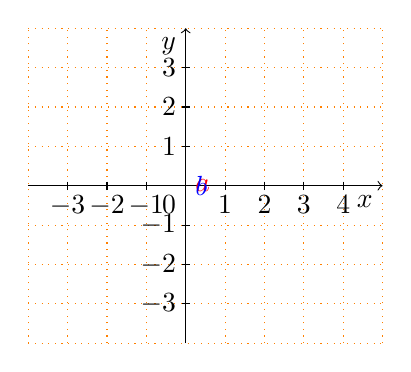
\begin{tikzpicture}[scale=.5, x=10mm, y=10mm]
    \draw[dotted,color=orange] (-4,-4) grid (5,4);
    \draw[->] (-4,0) -- (5,0) node[below left] {$x$};
    \draw[->] (0,-4) -- (0,4) node[below left] {$y$};
    
\foreach \x/\xtext in {-3/-3,-2/-2,-1/-1,1/1,2/2,3/3,4/4,}
\node[below]  at (\x,0) {$\xtext$};
\foreach \y/\ytext in {-3/-3,-2/-2,-1/-1,1/1,2/2,3/3}
\node[left] at (0,\y) {$\ytext$};

\foreach \xi in {-3,-2,...,4}
\draw (\xi,3pt) -- (\xi,-3pt);
\foreach \yi in {-3,-2,...,3}
\draw (3pt,\yi) -- (-3pt,\yi);

\node [below left] at (0,0) {0};
\draw[color=red,domain=-1.5:4.2] plot[id=x] function{(2*x-7)/3} 
        node[right] {$a$};
    
\draw[color=blue,domain=-3.5:4.2] plot[id=x] function{(2*x-3)/3} 
        node[right] {$b$};
\end{tikzpicture}
\caption{Esempio~23.17}\label{fig:23.1}
\end{inaccessibleblock}
\end{minipage}\hfill
\begin{minipage}{0.5\textwidth}
\centering
\begin{inaccessibleblock}[Esempio~23.18: due rette coincidenti]
% (c) 2012 Dimitrios Vrettos - d.vrettos@gmail.com
\begin{tikzpicture}[scale=.7, x=10mm, y=10mm]
    \draw[dotted,color=orange] (-4,-4) grid (5,3);
    \draw[->] (-4,0) -- (5,0) node[below left] {$x$};
    \draw[->] (0,-4) -- (0,3) node[below left] {$y$};
    
\foreach \x/\xtext in {-3/-3,-2/-2,-1/-1,1/1,2/2,3/3,4/4,}
\node[below]  at (\x,0) {$\xtext$};
\foreach \y/\ytext in {-3/-3,-2/-2,-1/-1,1/1,2/2}
\node[left] at (0,\y) {$\ytext$};

\foreach \xi in {-3,-2,...,4}
\draw (\xi,3pt) -- (\xi,-3pt);
\foreach \yi in {-3,-2,...,2}
\draw (3pt,\yi) -- (-3pt,\yi);

\node [below left] at (0,0) {0};
\draw[color=red,domain=-3.5:4.5] plot[id=x] function{-(2*x+1)/3} 
        node[right] {$a=b$};
\end{tikzpicture}
\caption{Esempio~23.18}\label{fig:23.2}
\end{inaccessibleblock}
\end{minipage}
\end{figure}
 \end{esempio}
 % \end{exrig}

 \vspace{-24pt}

% \ovalbox{\risolvii \ref{ese:22.39}, \ref{ese:22.40}, \ref{ese:22.41}, 
% \ref{ese:22.42}, \ref{ese:22.43}}

% \section{Sistemi fratti}
% \label{sec:22_fratti}
% 
% Nel seguente sistema
% 
% $\left\{\begin{array}{l}\frac{2}{x+1}-\frac{3}{y-2}=\frac{2x-5y+4}{xy+y-2-2x}
% \\3y+2(x-y-1)=5x-8(-x-2y+1)\end{array}\right.$
% di due equazioni in due incognite, la prima equazione presenta le
% incognite anche al denominatore.
% 
% \begin{definizione}
% Si chiama \emph{sistema fratto o frazionario} il sistema in cui almeno in una 
% delle equazioni che lo
% compongono compare l'incognita al denominatore.
% \end{definizione}
% 
% Poiché risolvere un sistema significa determinare tutte le coppie
% ordinate che verificano entrambe le equazioni, nel sistema fratto
% dovremo innanzi tutto definire il Dominio o Insieme di Definizione nel
% quale individuare le coppie soluzioni.
% 
% \begin{definizione}
% Si chiama \emph{Dominio}~($D$) o \emph{Insieme di Definizione}~($ID$) del 
% sistema fratto,
% l'insieme delle coppie ordinate che rendono diverso da zero i denominatori che
% compaiono nelle equazioni.
% \end{definizione}
% 
% % \begin{exrig}
%  \begin{esempio}
% 
% 
% $\longarray\left\{\begin{array}{l}\dfrac{2}{x+1}-\dfrac{3}{y-2}=\dfrac{2x-5y+4}{
% xy+y-2-2x}\\3y+2(x-y-1)=5x-8(-x-2y+1)\end{array}\right.$
% 
% \paragraph{Passo I} Scomponiamo i denominatori nella prima equazione
% per determinare il~$\mcm$.
% 
% 
% \[\longarray\left\{\begin{array}{l}{\dfrac{2}{x+1}-\dfrac{3}{y-2}=\dfrac{2x-5y+4
% }{(x+1)(y-2)}}\\{3y+2(x-y-1)=5x-8(-x-2y+1)}\end{array}
% \right.\Rightarrow\mcm=(x+1)(y-2).\]
% 
% \paragraph{Passo II} Poniamo le Condizioni di Esistenza da cui determineremo 
% il Dominio del
% sistema:
% \[\CE:\left\{\begin{array}{l}
%    x\neq -1\\y\neq~2
%    \end{array}\right.\Rightarrow D=\IS=\left\{(x;y)\in 
% \insR\times\insR\left|x\right.\neq -1\text{ e }y\neq~2\right\}.\]
% 
% \paragraph{Passo III} Riduciamo allo stesso denominatore la prima
% equazione, svolgiamo i calcoli nella seconda per ottenere la forma
% canonica:~$\left\{\begin{array}{l}{-5x+7y=11}\\{11x+15y=6}\end{array}\right.$
% 
% \paragraph{Passo IV} Risolviamo il sistema e otteniamo la coppia
% soluzione~$\left(-{\frac{123}{152};\frac{151}{152}}\right)$ che è
% accettabile.
%  \end{esempio}
% 
%   \begin{esempio}
% 
% 
% $\longarray\left\{\begin{array}{l}{\dfrac{3x+y-1}{x}=3}\\{\dfrac{2x+3y}{y-1}=7}
% \end{array}\right.$
% 
% \paragraph{Passo I} Per la prima equazione si ha~$\mcm=x$ per la 
% seconda~$\mcm=y-1$.
% 
% \paragraph{Passo II} Poniamo le Condizioni di Esistenza da cui determineremo 
% il Dominio:
% \[\CE:\left\{\begin{array}{l}
%    x\neq~0\\y\neq~1
%    \end{array}\right.\rightarrow D=\IS=\left\{(x;y)\in \insR\times\insR 
% |x\neq~0\text{ e }y\neq~1\right\}.\]
% 
% \paragraph{Passo III} Riduciamo allo stesso denominatore sia la prima che la 
% seconda equazione:
% $\left\{\begin{array}{l}{3x+y-1=3x}\\{2x+3y=7y-7}\end{array}\right.$
% 
% \paragraph{Passo IV} Determiniamo la forma canonica:
% $\left\{\begin{array}{l}{y-1=0}\\{2x-4y=-7}\end{array}\right.$
% 
% \paragraph{Passo V} Determiniamo con un qualunque metodo la coppia
% soluzione:~$\left(-{\frac{3}{2};1}\right)$ che non accettabile
% poiché contraddice la~$\CE$ e quindi non appartiene al dominio. Il
% sistema assegnato è quindi impossibile~$\IS=\emptyset $.
%  \end{esempio}
% % \end{exrig}
% 
% % \ovalbox{\risolvii \ref{ese:22.44}, \ref{ese:22.45}, \ref{ese:22.46}, 
% \ref{ese:22.47}, \ref{ese:22.48}, \ref{ese:22.49}}
% 
% \section{Sistemi letterali}
% \label{sec:22_letterali}
% 
%  \begin{definizione}
%  Si chiama \emph{sistema letterale} il sistema in cui
% oltre alle incognite, solitamente indicate con~$x$ e~$y$, compaiono altre
% lettere dette parametri.
%  \end{definizione}
% 
% 
% Distinguiamo tre casi distinti di discussione.
% 
% \subsection*{Le equazioni sono lineari e il parametro si trova solo al 
% numeratore}
% 
% % \begin{exrig}\vspace{1.10ex}
%  \begin{esempio}
%  $\left\{\begin{array}{l}{2ax-(a-1)y=0}\\{-2x+3y=a}\end{array}\right.$
% 
% 
% È un sistema letterale in quanto, reso in forma
% canonica, presenta un parametro nei suoi coefficienti. Esso è
% lineare, pertanto la coppia soluzione, se esiste, dipenderà dal
% valore del parametro.
% 
% Per \emph{discussione del sistema letterale} s'intende
% l'analisi e la ricerca dei valori che attribuiti al
% parametro rendono il sistema determinato (in tal caso si determina la
% soluzione) ma anche scartare i valori del parametro per cui il sistema
% è impossibile o indeterminato.
% Per discutere il sistema usiamo il metodo di Cramer.
% 
% \paragraph{Passo I} Calcoliamo il determinante del sistema:
% \[D=\left|\begin{array}{cc}{2a}&{-(a-1)}\\{-2}&{3}\end{array}\right|=4a+2.\]
% 
% \paragraph{Passo II} Determiniamo il valore del parametro che
% rende~$D$ diverso da zero:~$4a+2\neq~0\Rightarrow a\neq~0-\frac{1}{2}$. 
% Se~$a\neq -{\frac{1}{2}}$ il sistema è
% determinato.
% 
% \paragraph{Passo III} Calcoliamo i determinanti~$D_{x}$
% e~$D_{y}$ per trovare la coppia soluzione.
% \[D_{x}=\left|\begin{array}{cc}{0}&{-(a-1)}\\{a}&{3}\end{array}\right|=a\cdot 
% (a-1);\quad
% D_{y}=\left|\begin{array}{cc}{2a}&{0}\\{-2}&{a}\end{array}\right|=2a^{2}.\]
% Quindi~$x=\frac{a\cdot (a-1)}{4a+2}$ e~$y=\frac{2a^{2}}{4a+2}$.
% 
% \paragraph{Passo IV} Il determinante è nullo se~$a=-{\frac{1}{2}}$ poiché per 
% questo valore di~$a$ i
% determinanti~$D_{x}$ e~$D_{y}$ sono diversi da zero si ha che 
% per~$a=-{\frac{1}{2}}$ il sistema
% è impossibile.
% 
% Riassumendo si ha:
% \begin{center}
%  \begin{tabular}{lll}
% \toprule
% Condizioni sul parametro & Insieme Soluzione & Sistema\\
% \midrule
% $a\neq -{\frac{1}{2}}$ & $\left(\frac{a\cdot 
% (a-1)}{4a+2};\frac{2a^{2}}{4a+2}\right)$ & determinato\\
% $a=-{\frac{1}{2}}$ & $\emptyset $ & impossibile\\
% \bottomrule
% \end{tabular}
% \end{center}
%  \end{esempio}
% % \end{exrig}
% 
% \subsection*{Il parametro compare al denominatore in almeno una equazione del 
% sistema}
% 
% % \begin{exrig}\vspace{1.10ex}
% \begin{esempio}
%  $\longarray\left\{\begin{array}{l}{\dfrac{y+a}{3}-\dfrac{a-x}{a-1}=a}\\
%  {\dfrac{x+2a}{a}-3=\dfrac{y}{2}-a}\end{array}\right.$
% 
% Il sistema non è fratto pur presentando termini frazionari nelle sue
% equazioni; la presenza del parametro al denominatore ci obbliga ad
% escludere dall'insieme~$\insR$ quei valori che annullano il
% denominatore.
% Se~$a=1$ oppure~$a=0$ ciascuna equazione del sistema è priva di
% significato, pertanto lo è anche il sistema.
% Con le condizioni di esistenza~$\CE: a\neq~1$ e~$a\neq~0$
% possiamo ridurre allo stesso denominatore ciascuna equazione e condurre
% il sistema alla forma
% 
% canonica:~$\left\{\begin{array}{l}{3x+(a-1)y=2a^{2}+a}\\{2x-ay=2a-2a^{2}}\end{
% array}\right.$
% 
% 
% \paragraph{Passo I} Calcoliamo il determinante del sistema:
% $D=\left|\begin{array}{cc}{3}&{a-1}\\{2}&{-a}\end{array}\right|=2-5a.$
% 
% \paragraph{Passo II} Determiniamo il valore del parametro che
% rende~$D$ diverso da zero:~$2-5a\neq~0\Rightarrow a\neq \frac{2}{5}$
% Se~$a\neq \frac{2}{5}$ il sistema è determinato.
% 
% \paragraph{Passo III} Calcoliamo i determinanti~$D_{x}$
% e~$D_{y}$ per trovare la coppia soluzione
% 
% 
% \[D_{x}=\left|\begin{array}{cc}{2a^{2}+a}&{a-1}\\{2a-2a^{2}}&{-a}\end{array}
% \right|=a\cdot (2a-5);\quad
% 
% D_{y}=\left|\begin{array}{cc}{3}&{2a^{2}+a}\\{2}&{2a-2a^{2}}\end{array}
% \right|=2a\cdot (2-5a).\]
% Quindi~$x=\frac{a\cdot (2-5a)}{2-5a}$ e~$y=\frac{2a\cdot (2-5a)}{2-5a}$ e 
% semplificando~$(a;2a)$.
% 
% \paragraph{Passo IV} Il determinante è nullo se
% $a=\frac{2}{5}$ poiché anche i determinanti~$D_{x}$ e~$D_{y}$ si annullano si 
% ha
% per~$a=\frac{2}{5}$ sistema indeterminato.
% 
% Riassumendo si ha:
% 
% \begin{center}
% \begin{tabular}{lll}
% \toprule
% Condizioni sul parametro & Insieme Soluzione & Sistema\\
% \midrule
% $a=0\vee a=1$ & $\emptyset $ & privo di significato\\
% $a\neq \frac{2}{5}$ e~$a\neq~1$ e~$a\neq~0$ & $\left\{(a;2a)\right\}$ & 
% determinato\\
% $a=\frac{2}{5}$ & $\{\forall(x;y)\in\insR^2/3x-\frac{3}{5}y=\frac{18}{25}\}$ 
% & 
% indeterminato\\
% \bottomrule
% \end{tabular}
% \end{center}
% \end{esempio}
% % \end{exrig}
% \subsection*{Il sistema è frazionario}
% 
% % \begin{exrig}
%  \vspace{1.10ex}
%  \begin{esempio}
% $\left\{\begin{array}{l}\frac{y-a}{x}=\frac{2}{a}\\{x+y=1}\end{array}\right.$
% 
% Il sistema letterale è fratto e nel denominatore oltre al parametro
% compare l'incognita~$x$. Se~$a=0$ la prima equazione, e di conseguenza tutto 
% il sistema, è
% privo di significato. Per poter procedere alla ricerca
% dell'Insieme Soluzione poniamo sul
% parametro la condizione di esistenza:
% \begin{equation}
% \label{eq:23.1}
% \CE: a\neq~0.
% \end{equation}
% 
% Essendo fratto dobbiamo anche stabilire il Dominio del sistema:
% \begin{equation}
%  \label{eq:23.2}
% D=\{(x;y)\in \insR\times \insR | x\neq~0\}.
%  \end{equation}
% 
% 
% \paragraph{Passo I} Portiamo nella forma canonica:
% $\left\{\begin{array}{l}-2x+ay=a^{2}\\x+y=1\end{array}\right.\text{ con 
% }a\neq~0\text{ e }x\neq~0$.
% \paragraph{Passo II} Calcoliamo il determinante del sistema:
% $D=\left|\begin{array}{cc}{-2}&{a}\\{1}&{1}\end{array}\right|=-2-a=-(2+a)$.
% 
% \paragraph{Passo III} Determiniamo il valore del parametro che
% rende~$D$ diverso da zero:~$-2-a\neq~0\Rightarrow a\neq -2$.
% Se~$a\neq -2$ il sistema è determinato.
% \paragraph{Passo IV} calcoliamo i determinanti~$D_{x}$
% e~$D_{y}$ per trovare la coppia soluzione
% 
% \[D_{x}=\left|\begin{array}{cc}a^{2}&{a}\\{1}&{1}\end{array}\right|=a\cdot 
% (a-1);\quad
% D_{y}=\left|\begin{array}{cc}-2&a^{2}\\1& 
% 1\end{array}\right|=-2-a^{2}=-(2+a^{2}).\]
% Quindi~$x=-{\frac{a\cdot (a-1)}{2+a}}$ e~$y=\frac{a^{2}+2}{2+a}$ è la coppia 
% soluzione accettabile
% se~$x=-{\frac{a\cdot (a-1)}{2+a}}\neq~0$ per quanto stabilito 
% in~\ref{eq:23.2}; essendo~$a\neq~0$
% per la~\ref{eq:23.1} la coppia soluzione è accettabile se~$a\neq~1$.
% 
% \paragraph{Passo V} il determinante~$D$ è nullo se~$a=-2$
% essendo i determinanti~$D_{x}$ e~$D_{y}$ diversi
% da zero si ha:
% se~$a=-2$ il sistema è impossibile.
% Riassumendo si ha:
% 
% \begin{center}
% \begin{tabularx}{.9\textwidth}{XXll}
% \toprule
% Parametro & Incognite & Insieme Soluzione & Sistema\\
% \midrule
%  & $x\neq~0$ & & \\
%  $a=0$ & & & privo di significato\\
%  $a \neq2,a\neq0$ & & $\left(-{\frac{a\cdot 
% (a-1)}{2+a}};\frac{a^{2}+2}{2+a}\right)$ & determinato\\
%  $a\neq -2$ e~$a\neq~0$ e~$a\neq~1$ & & accettabile & \\
% $a=-2$ & & & impossibile\\
% \bottomrule
% \end{tabularx}
% \end{center}
%  \end{esempio}
% % \end{exrig}
% 
% % \ovalbox{\risolvii \ref{ese:22.50}, \ref{ese:22.51}, \ref{ese:22.52}, 
% \ref{ese:22.53}, \ref{ese:22.54}, \ref{ese:22.55}, \ref{ese:22.56}}

\section{Sistemi lineari di tre equazioni in tre incognite}
\label{sec:compl1_sistemitreeq}

% \begin{problema}
% Determinare tre numeri reali~$x, y, z$ (nell'ordine) tali
% che il doppio del primo uguagli l'opposto del secondo,
% la differenza tra il primo e il triplo del terzo sia nulla e la somma
% del secondo con il terzo superi il primo di~4 unità.
% \end{problema}

\begin{problema}
Determinare tre numeri reali~$x, y, z$ (nell'ordine) tali
che il doppio del primo uguagli l'opposto del secondo,
il triplo del terzo sia uguale al primo aumentato~$4$
e che la somma del secondo con il terzo sia inferiore al primo di~$12$ unità.
\end{problema}

\begin{soluzione}
Formalizziamo le condizioni espresse nel testo attraverso equazioni
lineari:

\begin{enumeratea}
\item il doppio del primo uguagli l'opposto del secondo:~$2x=-y$
\item il triplo del terzo sia uguale al primo aumentato~$4$:~$3z=x+4$
\item la somma del secondo con il terzo sia inferiore al primo di~$12$ 
unità:~$y+z=x-12$.
\end{enumeratea}

Le tre condizioni devono essere vere contemporaneamente, quindi i tre
numeri sono la terna soluzione del sistema di primo grado di tre equazioni in 
tre incognite:
\[\left\{\begin{array}{l}
  2x=-y\\
  3z=x+4\\
  y+z=x-12
\end{array}\right.\]

Per prima cosa scriviamo il sistema in forma normale:
\[\left\{\begin{array}{l}
  2x+y=0\\
  -x+3z=4\\
  -x+y+z=-12
\end{array}\right.\]

Possiamo ora ricavare la~$y$ dalla prima equazione e sostituirla nelle altre 
due:
\[\left\{\begin{array}{l}
  y=-2x\\
  -x+3z=4\\
  -x -2x+z=-12
\end{array}\right.
\Rightarrow
\left\{\begin{array}{l}
  y=-2x\\
  -x+3z=+4\\
  -3x+z=-12
\end{array}\right.\]

In questo modo abbiamo ottenuto un sottosistema formato da due equazioni in 
due incognite:
\[\left\{\begin{array}{l}
  -x+3z=+4\\
  -3x+z=-12
\end{array}\right.\]

Possiamo risolverlo facilmente con il metodo di riduzione:

\[\left\{\begin{array}{l}
  3x-9z=-12\\
  -3x+z=-12
\end{array}\right.
\Rightarrow -8z=-24 \Rightarrow z=3
\qquad
\left\{\begin{array}{l}
  -x+3z=+4\\
  9x-3z=+36
\end{array}\right.
\Rightarrow 8x=40 \Rightarrow x=5
\]

Risolto così il sottosistema possiamo risolvere il sistema di partenza:
\[\left\{\begin{array}{l}
  x=5\\
  y=-2x=-10\\
  z=3
\end{array}\right.\]

\end{soluzione}

% \begin{exrig}
 \begin{esempio}
$\left\{\begin{array}{l}3x+y-z=7\\x+3y+z=5\\x+y-3z=3\end{array}\right.$

Procediamo con il metodo di riduzione. Sommiamo le prime due 
equazioni:~$4x+4y=12$
Moltiplichiamo la seconda equazione per~3 e sommiamo con la 
terza:~$3(x+3y+z)+x+y=3\cdot 5+3=4x+10y=18$.
Costruiamo il sistema di queste due equazioni
nelle sole due incognite~$x$ e~$y$:
$\left\{\begin{array}{l}4x+4y=12\\4x+10y=18\end{array}\right..$

Moltiplichiamo la seconda equazione per~$-1$ e sommiamo le due equazioni:
\begin{align*}
\left\{\begin{array}{l}4x+4y=12 \\-4x-10y=-18
\end{array}\right.&\Rightarrow
\left\{\begin{array}{l}4x+4y=12
\\-4x-10y+4x+4y=-18+12 \end{array}\right.\\
&\Rightarrow
\left\{\begin{array}{l}4x+4y=12 \\-6y=-6\Rightarrow
y=1 \end{array}\right.\Rightarrow
\left\{\begin{array}{l}x=2 \\y=1
\end{array}\right..
\end{align*}

Sostituendo nella prima equazione del sistema ricaviamo la terza
incognita:~$\left\{\begin{array}{l}x=2\\y=1\\z=0\end{array}\right.$.

La terna soluzione del sistema assegnato è~$(2;1;0)$.
 \end{esempio}
% \end{exrig}

% \ovalbox{\risolvii \ref{ese:22.57}, \ref{ese:22.58}, \ref{ese:22.59}, 
% \ref{ese:22.60}, \ref{ese:22.61}, \ref{ese:22.62}, \ref{ese:22.63}}
% 
% \section{Sistemi da risolvere con sostituzioni delle variabili}
% \label{sec:22_sostituzione}
% 
% Alcuni sistemi possono essere ricondotti a sistemi lineari per mezzo di
% sostituzioni nelle variabili.
% 
% % \begin{exrig}
%  \begin{esempio}
% $\longarray\left\{\begin{array}{l}\dfrac{1}{x}+\dfrac{2}{y}=3\\\dfrac{2}{x}
% -\dfrac{4}{y}=-1 \end{array}\right.$
% 
% Con la seguente sostituzione di variabili
% \begin{align}
%  \label{eq:23.3}
% \longarray\left\{\begin{array}{l}
%     u=\dfrac{1}{x}\\
%     v=\dfrac{1}{y}
% \end{array}\right.
% \end{align}
% 
% il sistema diventa
%  \[\left\{\begin{array}{l}u+2v=3 \\2u-4v=-1 \end{array}\right.\]
% 
% Per risolverlo possiamo moltiplicare per~2 la prima equazione:
% \[\left\{\begin{array}{l}2u+4v=6 \\2u-4v=-1
% \end{array}\right.\]
% Sommando membro a membro abbiamo~$4u=5$ dalla
% quale possiamo determinare~$u=\frac{5}{4}$
% 
% Per ricavare l'incognita~$v$ moltiplichiamo la prima equazione per $-2$, 
% otteniamo
% \[\left\{\begin{array}{l}-2u-4v=-6 \\2u-4v=-1 \end{array}\right.\]
% Sommando membro a membro abbiamo
% \[-8v=-7\Rightarrow v=\frac{7}{8}.\]
% 
% Avendo trovato i valori delle incognite~$u$ e~$v$ possiamo ricavare~$x$ e~$y$ 
% sostituendo con i valori trovati nella~\ref{eq:23.3}:
% \[\longarray\left\{\begin{array}{l}\dfrac{5}{4}=\dfrac{1}{x}\\\dfrac{7}{8}
% =\dfrac{1}{y}\end{array}\right.\Rightarrow
% \left\{\begin{array}{l}x=\dfrac{4}{5}\\y=\dfrac{8}{7}\end{array}\right.\]
%  \end{esempio}
% % \end{exrig}

% \ovalbox{\risolvii \ref{ese:22.64}, \ref{ese:22.65}, \ref{ese:22.66}}
